\documentclass{article}
\usepackage[utf8]{inputenc}
\usepackage{graphicx}
\usepackage[margin=1in]{geometry}
\usepackage[dvipsnames]{xcolor}
\usepackage{url}
\usepackage{hyperref}
\usepackage[numbers]{natbib} % for numeric references
\usepackage{float}

\begin{document}

\begin{titlepage}
    \begin{center}
        \includegraphics[width=3cm]{figures/MSP-logo.jpg} 
        \vspace{1cm}
        
        
       {\Large\bfseries
        Patient Age and Tumor Size: A Correlation and Subsampling\\[0.3cm]
        Analysis
        \par}

        \vspace{0.6cm}

       {\large
       The Bioconductor MAINZ Breast Cancer Cohort
       \par}

        
        \vspace{1.5cm}
        
        \textbf{\Large Romy Wegmann (I6399818)}
        
        \vfill
        
        \large Date: \today
        
    \end{center}
\end{titlepage}

\newpage

\section*{Introduction}
Breast cancer accounts for a quarter of all female cancers ~\cite{Lorincz2020} leading to 694,000 deaths globally in 2024 ~\cite{WHO2026}. Histological classification of breast cancer tumors, including characteristics such as tumor grade, size, and hormone receptor status, play an important role in prognosis and treatment ~\cite{Lorincz2020}. Although breast cancer is more common in women above the age of 40, patients can range from 20 years old to over 90 ~\cite{Brown2026}. This project examines the correlation between patient age and tumor size in 200 patients from the MAINZ breast cancer cohort. 

\section*{Data sample and Methods}
The MAINZ breast cancer cohort is a publicly available dataset published through Bioconductor by Schroeder et al. in 2026 ~\cite{Schroeder2026}. The data was originally published by Schmidt et al. in 2008 ~\cite{Schmidt2008} and examined associations between tumor gene expression and subsequent outcomes such as metastasis. Alongside gene-expression data, the dataset also contains clinical annotations such as patient age (in years) and tumor size (in cm). Patient ages range from 25-90 years while tumor size ranges from 0.1-6 cm.

Based on this information, a scatter plot was created that plotted the correlation between patient age and tumor size. A linear regression line was fitted and Pearson's correlation coefficient was calculated to measure the strength and direction of the correlation. 

To investigate the effect of sample size, random subsamples of 20,40, 80 and 160 patients were drawn without replacement. These values double each time and should illustrate the effect of increasing sample size up to the original cohort size. For each sample size, patients were randomly selected from the full cohort and Pearson's correlation coefficient was calculated. This was repeated 1000 times for each sample size. The number of repeats provides sufficient values for comparison without requiring a lot of time. 

The resulting correlation estimates were displayed using boxplots, and their standard deviation was calculated and displayed to compare variability across different sample sizes.
\section*{Results and Discussion}

\subsection{Correlation Between Patient Age and Tumor Size}

\begin{figure}[H]
    \centering
    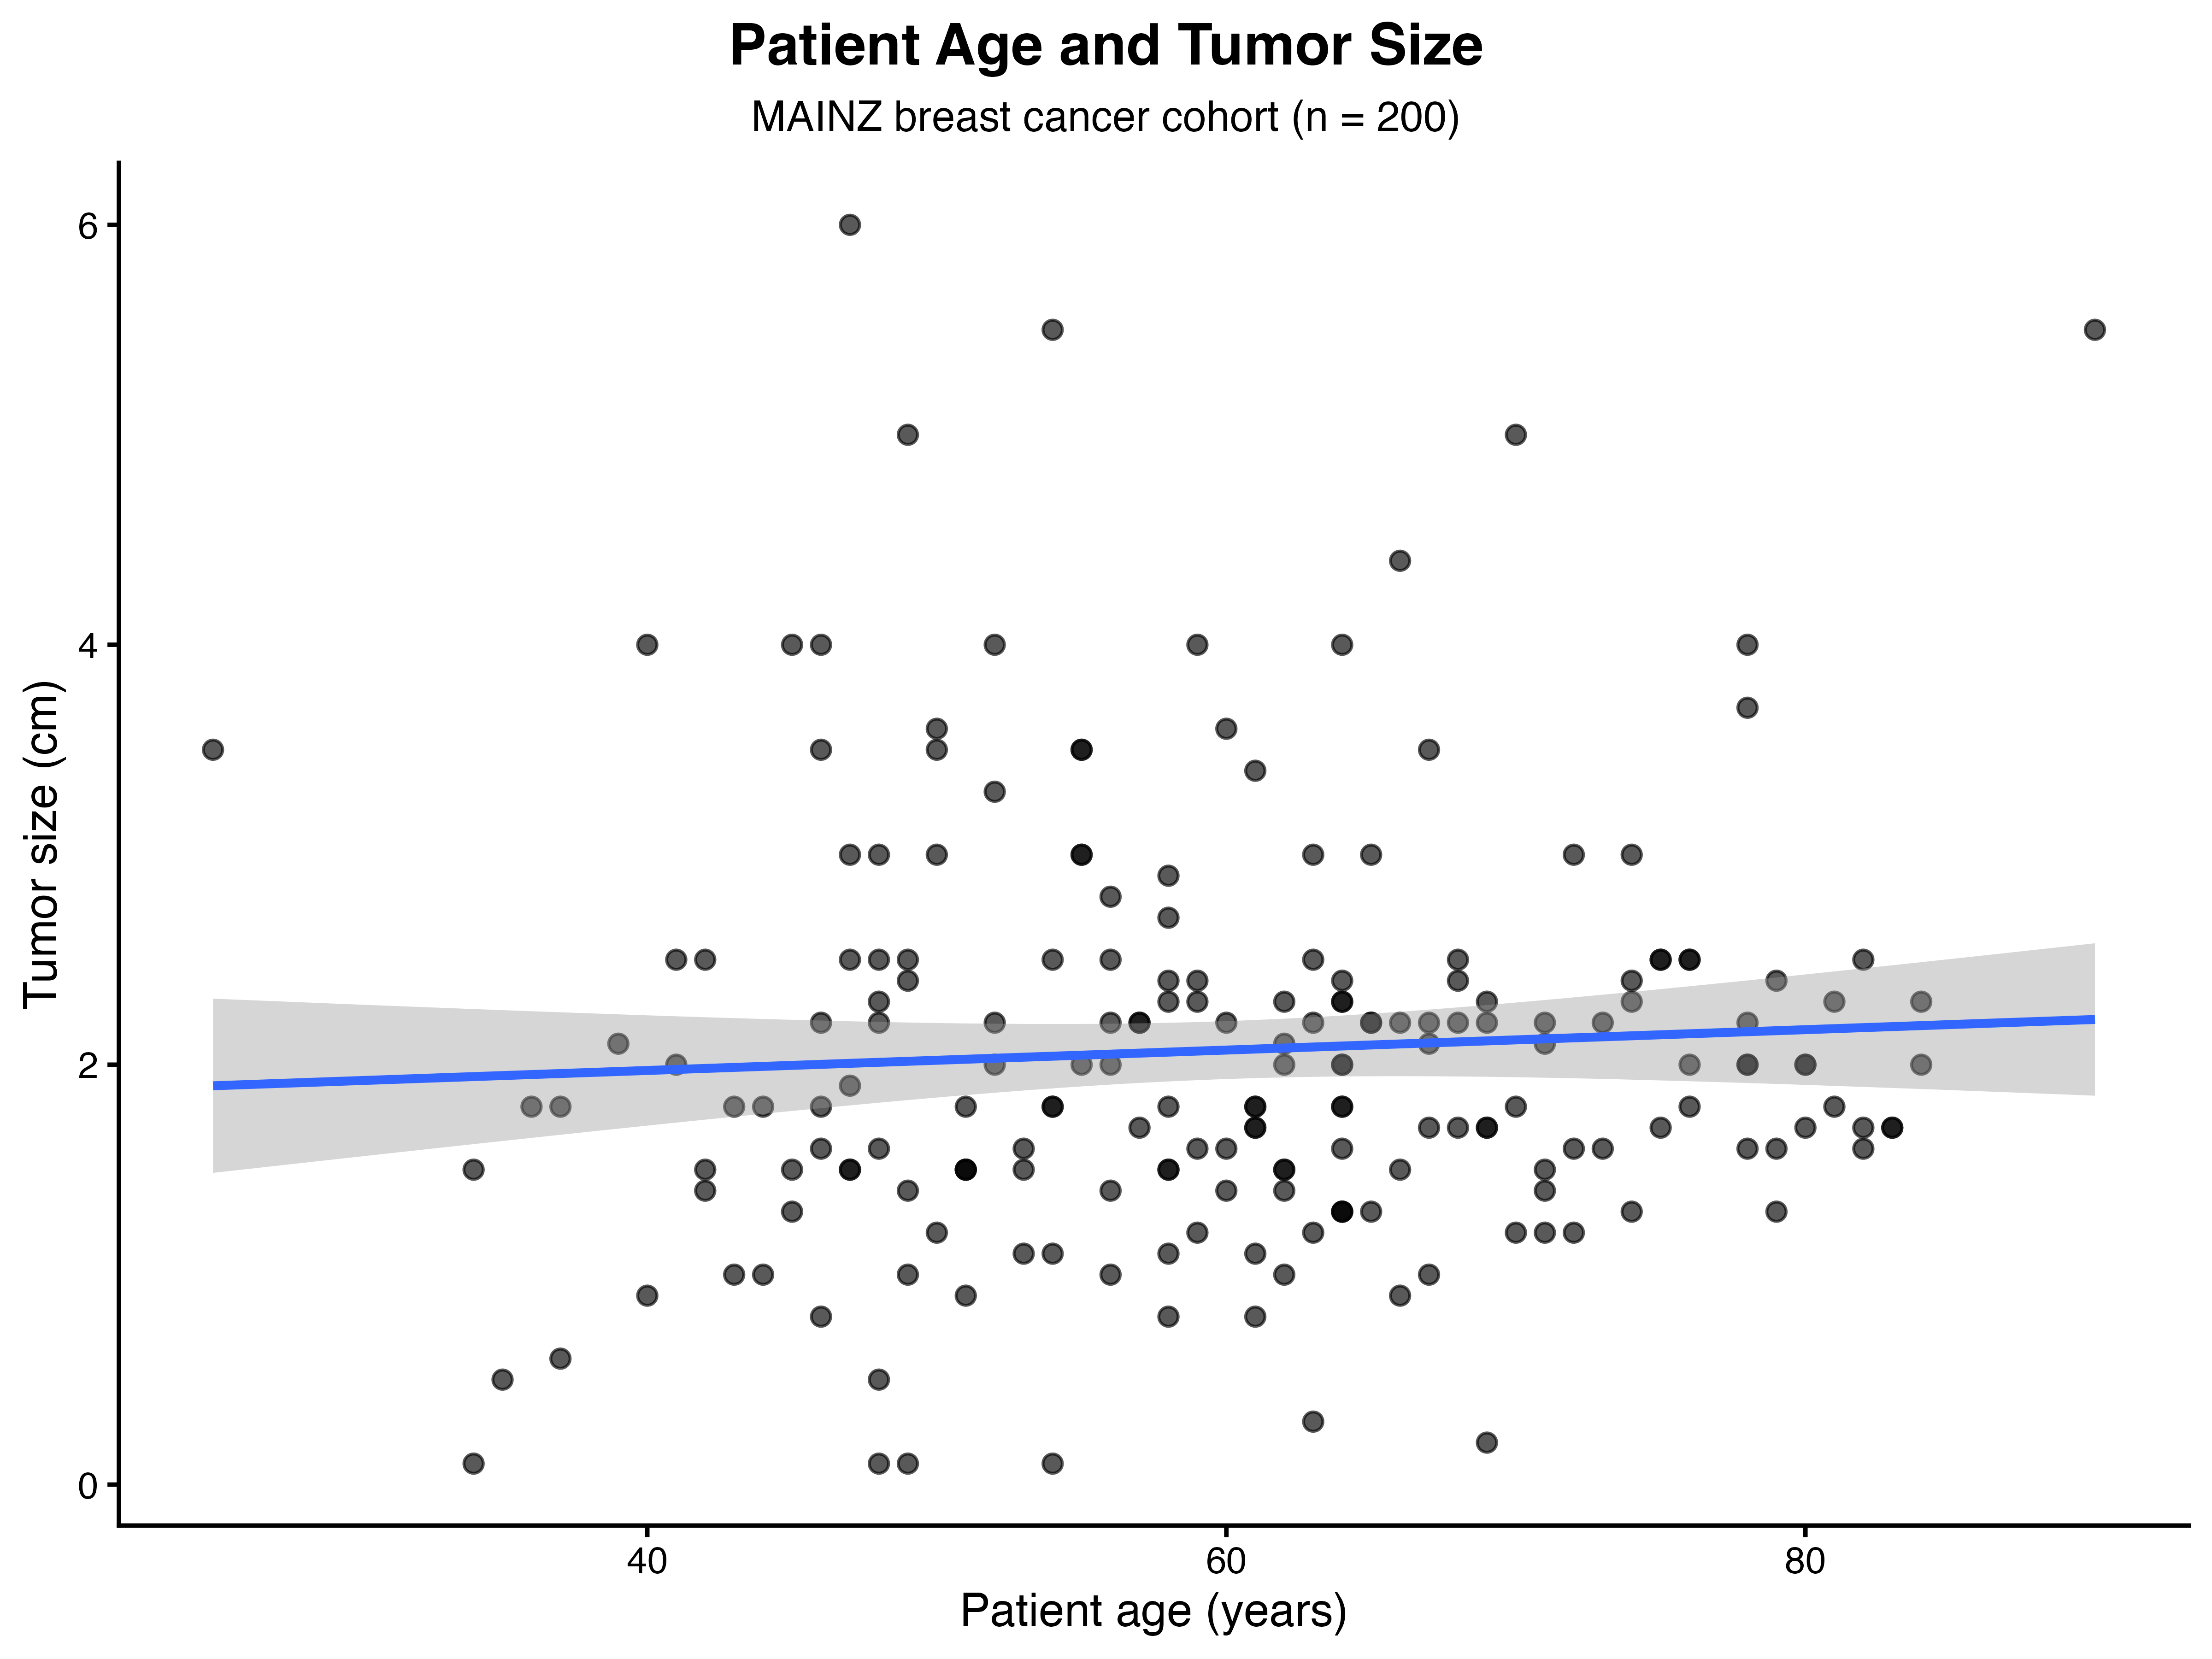
\includegraphics[
        width=0.65\textwidth,
        height=0.28\textheight,
        keepaspectratio
    ]{figures/Age_vs_Tumor_Size.png}
    \caption{Relationship between patient age and tumor size
    in the MAINZ breast cancer cohort}
    \label{fig:age_tumor}
\end{figure}

Figure 1 shows the relationship between patient age and tumor size with a fitted linear regression line. The data points are widely scattered, and the regression line is near horizontal. The Pearson's correlation coefficient obtained was r= 0.0607, indicating a very weak positive linear correlation. This suggests that patient age is not strongly associated with tumor size in this cohort. 

\subsection{Effect of Sample Size on Correlation Estimates}

\begin{figure}[H]
    \centering
    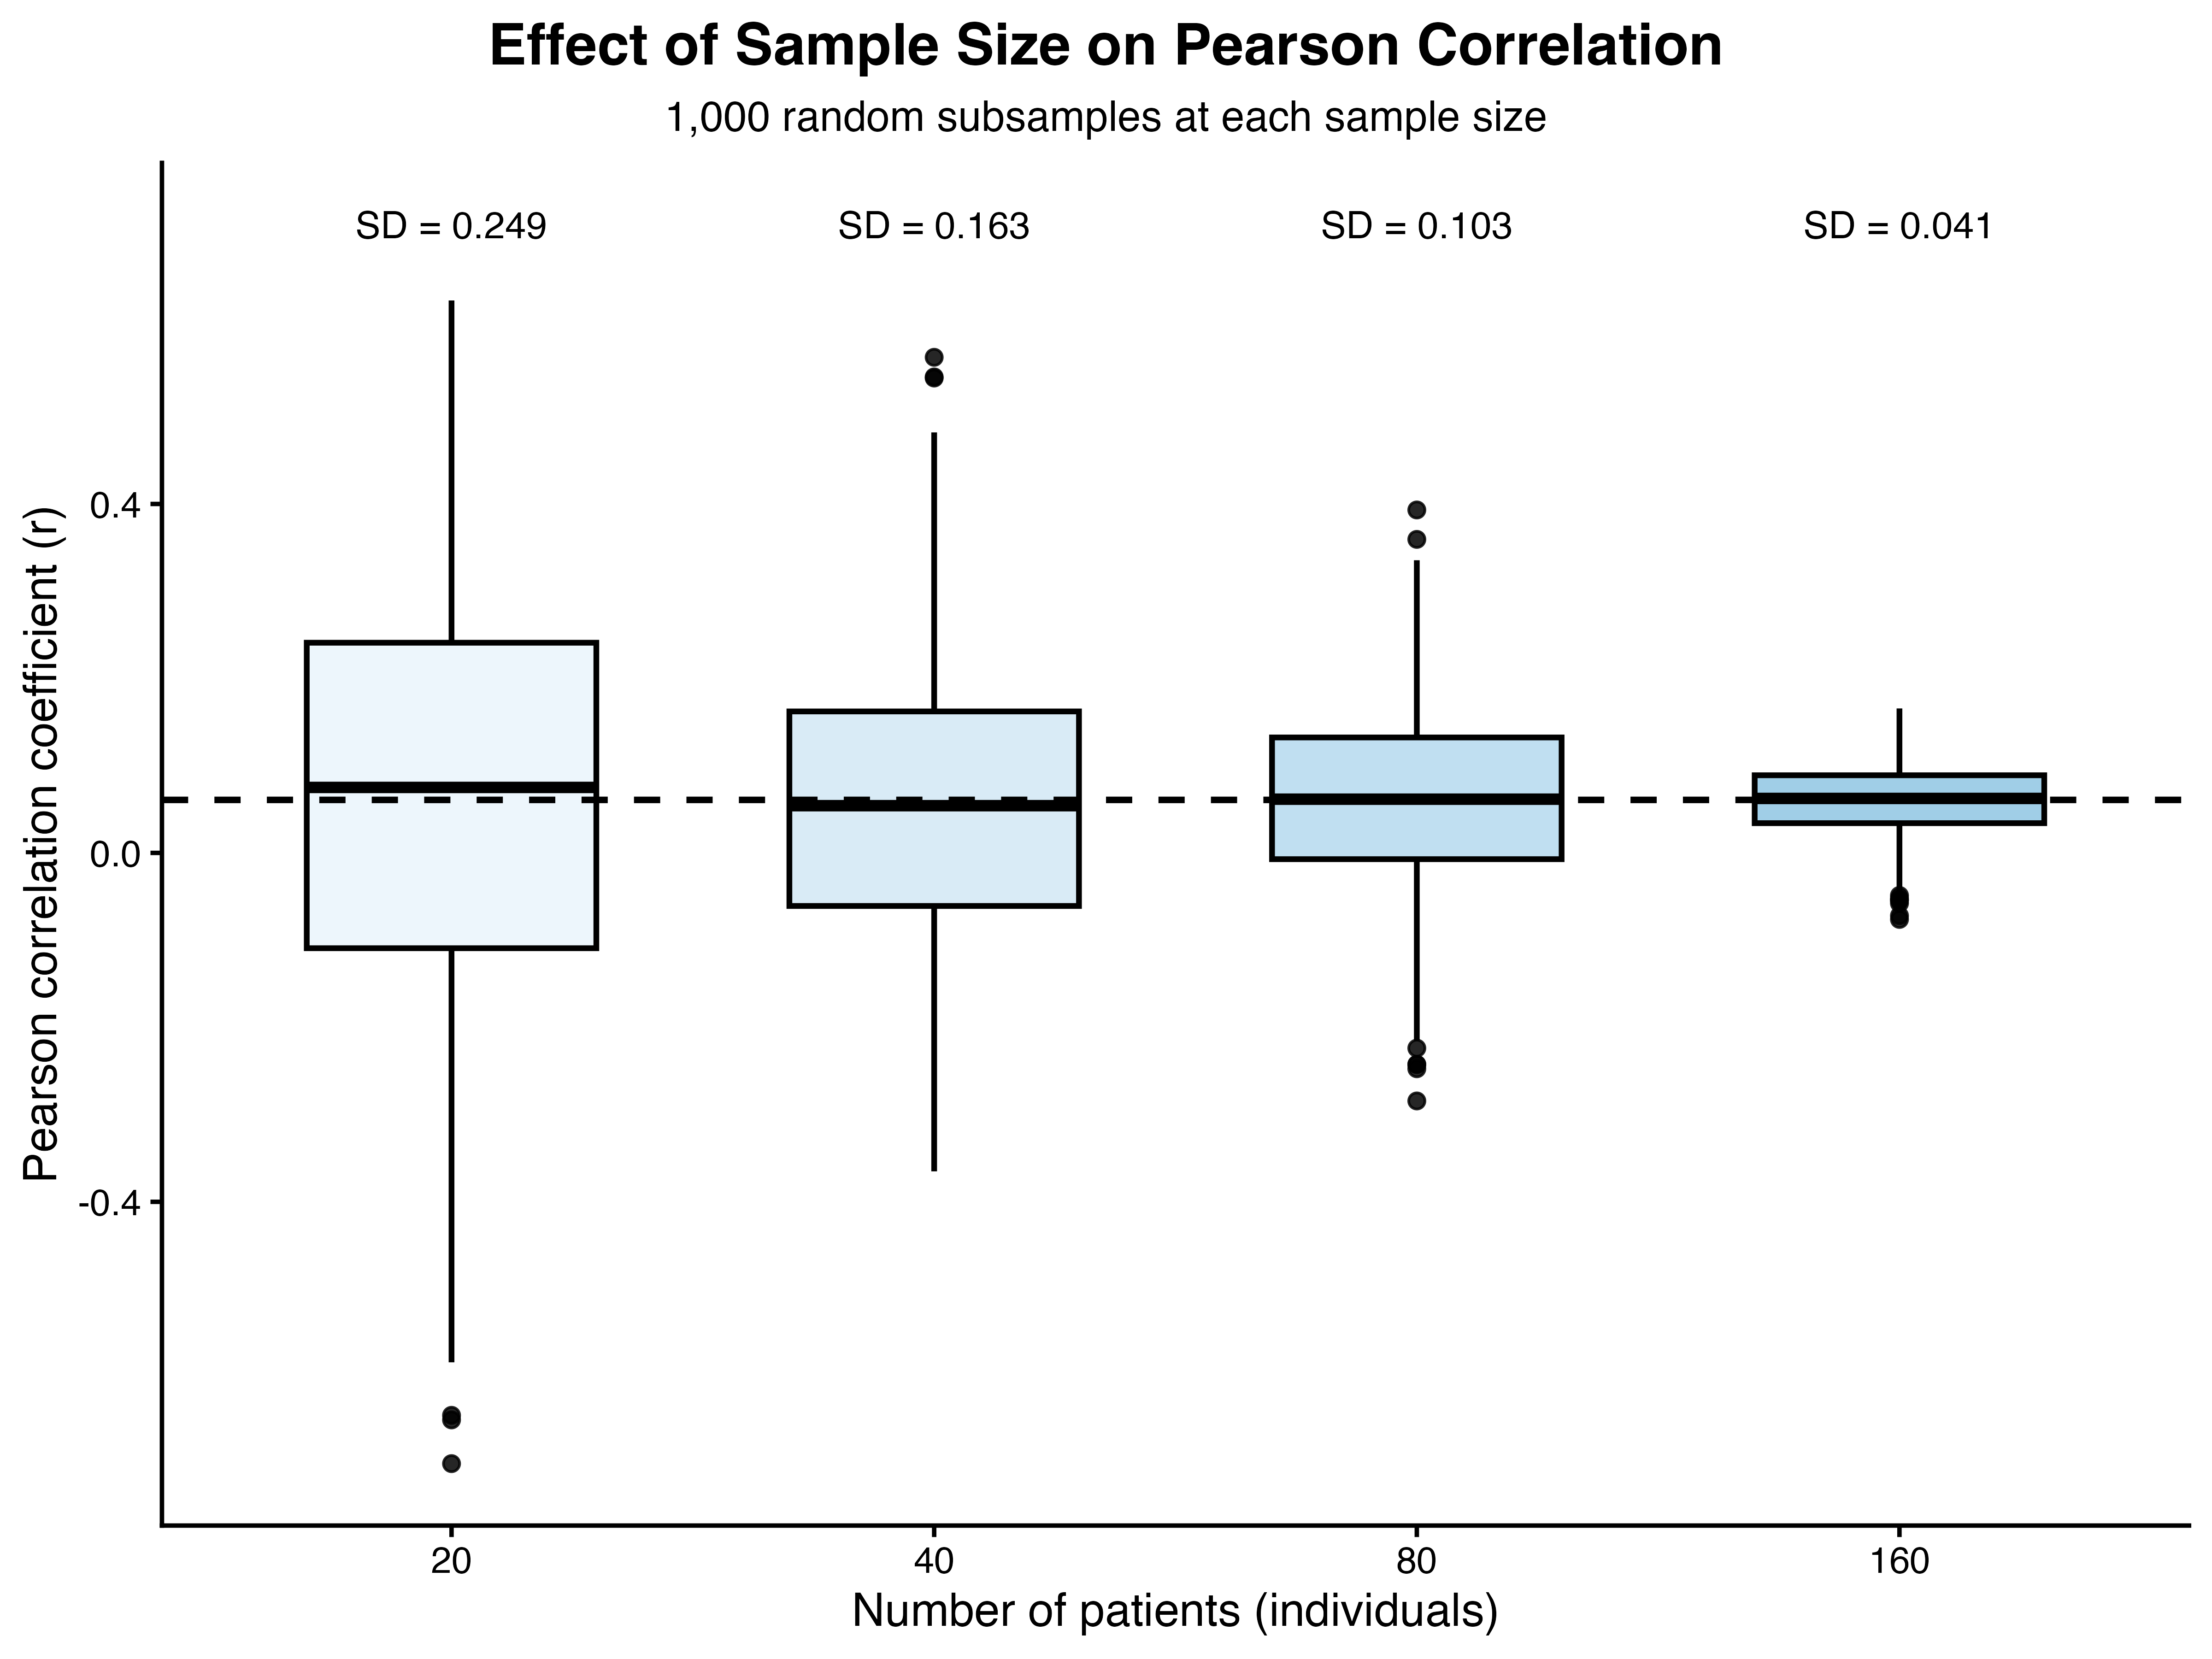
\includegraphics[
        width=0.65\textwidth,
        height=0.28\textheight,
        keepaspectratio
    ]{figures/Subsampling_Pearson_Correlation.png}
    \caption{Distribution of Pearson's correlation coefficients
    from 1000 random subsamples for each sample size
    (20, 40, 80, and 160 patients).
    The dashed horizontal line represents the correlation
    calculated using all 200 patients (r = 0.0607)}
    \label{fig:subsampling}
\end{figure}

Figure 2 shows how Pearson's correlation coefficient varies with increasing sample size. Smaller sample sizes produced a larger range of correlation estimates, while smaller sample sizes produced estimates closer to those of the full cohort. The standard deviation decreased from 0.249 to 0.041, indicating that larger sample sizes reduce sampling variability and produce more stable correlation estimates.

Larger sample sizes improve the stability of the statistical estimates and make them less sensitive to individual outliers. As sample sizes increase, estimates become more consistent, and reduce the risk of over-estimating the relationship observed. 

\begin{thebibliography}{9}

\bibitem{Lorincz2020}
L\H{o}rincz, K.-Z., Pap, Z., Mocan, S.,
L\H{o}rincz, C. E., \& Bar\'oti, B. (2020).
Ultrasound-guided core-needle biopsy of suspicious
breast lesions.
\textit{Journal of Interdisciplinary Medicine},
\textit{5}, 48--55.
\url{https://doi.org/10.2478/jim-2020-0010}

\bibitem{WHO2026}
World Health Organization. (2026, July 3).
\textit{Breast cancer}.
\url{https://www.who.int/news-room/fact-sheets/detail/breast-cancer}.

\bibitem{Brown2026}
Brown, J. (2026, October 5).
\textit{Breast cancer in young women: Signs, risks, and latest research}.
Breast Cancer Research Foundation.
\url{https://www.bcrf.org/about-breast-cancer/breast-cancer-young-women/}

\bibitem{Schroeder2026}
Schroeder, M., Haibe-Kains, B., Culhane, A.,
Sotiriou, C., Bontempi, G., \& Quackenbush, J. (2026).
\textit{breastCancerMAINZ: Gene expression dataset
published by Schmidt et al. [2008] (MAINZ)}.
Bioconductor.
\url{https://doi.org/10.18129/B9.bioc.breastCancerMAINZ}

\bibitem{Schmidt2008}
Schmidt, M., B\"ohm, D., von T\"orne, C.,
Steiner, E., Puhl, A., Pilch, H., Lehr, H. A.,
Hengstler, J. G., K\"olbl, H., \& Gehrmann, M. (2008).
The humoral immune system has a key prognostic
impact in node-negative breast cancer.
\textit{Cancer Research}, 68(13), 5405--5413.
\url{https://doi.org/10.1158/0008-5472.CAN-07-5206}


\end{thebibliography}
\end{document}